\section{Čtvrtá verze}

\subsection{Rozšíření elektroniky}

Čtvrtá verze byla co se elektroniky týče přímým pokračováním předchozí verze, kterou dále rozšiřuje.

Trezor získal oproti minulé verzi možnost komunikace pomocí IR z důvodu identifikace růz\-ných dveří, dále získal magnetický enkodér, pro možnost snaz\-ší\-ho ovládání %todo možnost 3x 
motoru zámku. 
Další inovací byl programovací systém s~USB-C, na místo USB-micro jako dřív. Nový programátor má možnost úplně si odpojit napáje\-ní, a to v rámci šetření 
energie, když trezor programátor nevyužívá. 
Zároveň umožňuje zákaz přeprogramování.

Podstatnou změnou také bylo rozdělení elektroniky do dvou různých desek, protože na jedné by nebyl dostatek místa. Jedna deska %todo odkaz na výkres do přílohy
 tak obsahuje  
kruh LED a čip LDC1614 nebo LDC1314 se čtyřmi cívkami, které měří vzdálenost tlakové desky. Na druhé desce  %todo odkaz na výkres do přílohy
je vše ostatní, tedy procesor, akcelerometr,
gyroskop, magnetický kompas, RTC (Real Time Clock, hodiny reálného času), barometr, IR vysílač a přijímač, magnetický enkodér, programátor, řešení 
napájení, řízení motoru a nabíječka. 


\subsection{Princip zamykání}

Na trezoru se dále změnily princip zamykání a ovládání. 

Důvodem změn bylo náročné uložení rotační západky, 
které vyžadovalo ozubený věnec a několik dalších tisknutých dílů.

Zamykání je založeno na mechanizmu bajonetu a zamčení je zajištěno západ\-kou, která zabraňuje zpětnému otočení.
Západka je ovládána motorem, který otáčí magnetem a přitahuje nebo odpuzuje magnet na západce. Důvodem pro magnetické ovládání
byla možnost západku ovládat i přes pevnou stěnu, a~také pružné spojení, které takto vznikne, takže se trezor například dá zavřít, i~když
je už zamčen (když například dveře nejsou dovřeny).

\begin{figure}[htbp]
    \centering
    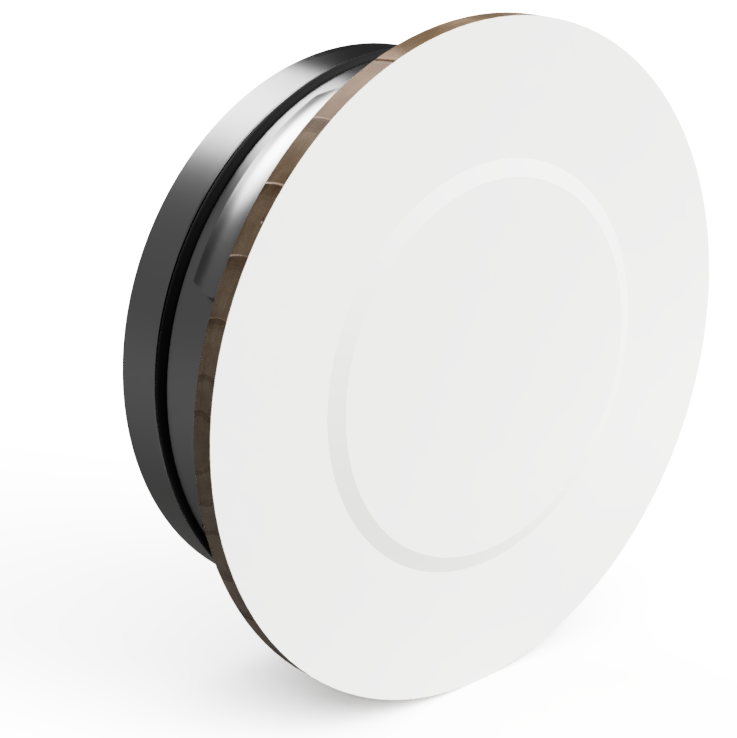
\includegraphics[width=170pt]{kapitoly/obrazky/E4/predni_render.png}
    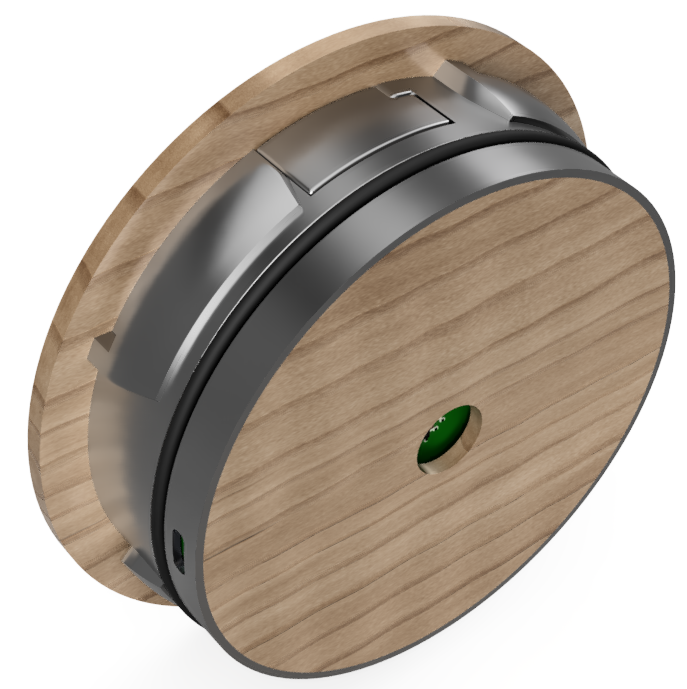
\includegraphics[width=170pt]{kapitoly/obrazky/E4/zadni_render.png}
    \caption{Rendery dveří trezoru E4 -- vlevo přední pohled, vpravo zadní pohled 	\centering}
    \label{fig:E4-render}
\end{figure}


\subsection{Ovládání}
Předchozí varianty měly jako hlavní ovládací prvek enkodér s tlačítkem, ten jsem v nynější variantě odstranil, aby přední stěna neměla tak velký 
výstupek. Proto jsem tento prvek nahradil indukční tlakovou deskou, která vyplnila vnitřek kruhu ledek. 
Zbytek ovládání víceméně přetrval, jen kvůli nedostatku času a pandemií způsobenému nedostatku součástek, trezor přišel o GPS. Na druhou stranu 
získal barometr s rozlišením schopným detekovat změnu výšky o půl metru.

\subsection{Napájení}
Předchozí verzím sloužila jako napájení powerbanka. Ta však kladla poměrné velké omezení, dokázala poskytnout proud pouze jednoho ampéru, a proto 
jsem jí nahradil vlastním zdrojem, dvěma bateriemi 18650. 
To  samozřejmě znamenalo nutnost vlastního řešení stabilizace napětí, díky čemuž 
trezor dostal stepup, který spíná napětí z 3,5~V až 4,2~V na 5~V, a původně stepdown, později lineární stabilizátor, který poskytuje 3,3~V. 
%todo konkrétní obvody 

Trezor také dostal vlastní nabíječku, aby pro nabíjení baterií stačilo připojit kabel, stejně jako třeba u mobilu.

